\documentclass[12pt]{article}
\usepackage[ngerman]{babel}
\usepackage{float}
\usepackage{graphicx}
\usepackage{hyperref}
\usepackage{cleveref}
\usepackage[%
  backend=biber,
  style=alphabetic,
  sorting=ynt]{biblatex}
\addbibresource{bib.bib}
\author{Maximilian Heim}
\crefname{section}{Kapitel}{Kapitel}
\title{Identitäts und Berechtigungsmanagement}
\begin{document}
\maketitle
\newpage
\tableofcontents
\newpage
\section{Einleitung}
\subsection{Aufgabenstellung}
Diese Seminararbeit wurde im Rahmen der Vorlesung IT-GRC angefertigt. Ziel der Arbeit ist es die in \cref{subsec:forschungsfragen} definierten Forschungsfragen zu beantworten. Die Forschungsfragen zielen darauf ab wichtige Aspekte des betrieblichen Identitäts- und Berechtigungsmanagements im Kontext der IT-GRC zu beleuchten.
\subsection{Forschungsfragen}
\label{subsec:forschungsfragen}
Im Rahmen der Seminararbeit wurden 7 Forschungsfragen definiert, diese sind im Folgenden aufgeführt.
\begin{itemize}
  \item Was versteht man unter den Begriffen \glqq{}Identität\grqq{} sowie \glqq{}Identitätsmanagement\grqq{} und welche Zielstellung wird dabei verfolgt?
  \item Was versteht man unter den Begriffen \glqq{}Berechtigung\grqq{} sowie \glqq{}Berechtigungsmanagement\grqq{} und welche Zielstellung wird dabei verfolgt?
  \item Welche Standards, Methoden, Technologien und Tools lassen sich differenzieren?
  \item Welche Aufgaben und Prozesse sind im Kontext von Identitäts und Berechtigungsmanagement zu bearbeiten?
  \item Welche betrieblichen Anwendungsfälle zeigen die Bedeutung des Identitäts und Berechtigungsmanagements auf?
  \item Wie wird das Identitäts und Berechtigungsmanagement im Kontext der Sicherheit in der Informationstechnik eingesetzt?
  \item Wer hat im Unternehmen typischerweise die Zuständigkeit für Identitäts und Berechtigungsmanagemnt und wer führt diese Aufgaben operativ durch?
\end{itemize}
\section{Grundlagen}
\label{sec:grundlagen}
\subsection{Einordnung}
Das Identitäts- und Berechtigungsmanagent ist eine zentrale Disziplin in der Informationssicherheit. Das Identitäts- und Berechtigungsmanagement besteht aus Richtlinien, Prozessen und Technologien welche das Risiko von unberechtigten Zugriffen minimieren sollen. Identitätsmanagement und Berechtigungsmanagement sind zwei unterschiedliche Disziplinen, jedoch werden diese meist zusammen angewendet. ~\cite{mohammed2017systematic} Es wird häufig zwischen Identitäts- und Berechtigungsmanagement (IAM) und Customer Identitäts- und Berechtigungsmanagement (CIAM) unterschieden. Bei IAM geht es um die Authentifikation und Zugriffskontrolle im Unternehmen. Im Kontrast behandelt das CIAM die Authentifikation und Zugriffskontrolle von Nutzern außerhalb vom Unternehmen.~\cite{mohammed2017systematic} ~\cite{liveretos2022customer}
\subsection{Identität}
Um den Begriff Identitätsmanagement zu definieren sollte zuerst der Begriff der Identität definiert werden. In der Philosophie wird Identität über die Ununterscheidbarkeit von Dingen definiert. Nach dem Identitätsprinzip sind zwei Dinge genau dann identisch wenn sich zwischen ihnen keine Unterschiede finden lassen. Hierbei geht es um die Fragestellung \glqq{}wer/was bist du?\grqq{}. Im Kontext des Identitätsmanagements handelt es sich hier um digitale Identitäten, d.h. eine Menge an Attributen und Rollen die einer Person, einem IT-System oder einer Anwendung zugeordnet werden können, inklusive einem Bezeichner und Zugangsdaten die zur Nutzung der Identität notwendig sind.~\cite{tsolkas2017} Ein Subjekt (Person, System) kann mehreren digitalen Identitäten zugeordnet sein. Dieser Sachverhalt ist in \cref{fig:identity} dargestellt.
\begin{figure}[H]
  \label{fig:identity}
  \centering
  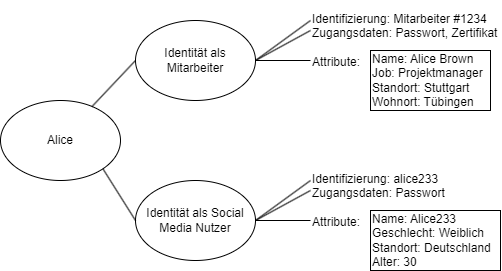
\includegraphics[width=0.9\textwidth]{assets/identity.png}
  \caption{Digitale Identität - In Anlehnung an: Grafik 2.1 aus Identity Management Concepts, Technologies, and Systems von Elisa Bertino und Kenji Takahashi}
\end{figure}
In der Informationstechnik wird der Beweis über die eigene Identität, basierend auf Bezeichner und Zugangsdaten als Authentifizierung bezeichnet. Es haben sich verschiedenste Authentifizierungsverfahren durchgesetzt von denen im Folgenden einige vorgestellt werden.
\paragraph{Authentifizierungsverfahren}
\begin{itemize}
  \item Passwörter und Pins sind die wohl bekanntesten Arten der Authentifizierung. Jedoch ist es auch eine der unsichersten Arten da diese gerne mehrfach verwendet werden oder bei unzureichender Länge geknackt werden können~\cite{tsolkas2017}
  \item Tokens sind eine andere Art der Authentifizierung die auf Besitz und Wissen basieren und daher sicherer sind wie rein wissensbasierte Verfahren wie Passwörter. Hierbei wird ein Gerät verwendet welches nach Entsperrung mittels Pin/Passwort ein Einmalpasswort ausgibt oder automatisch die Authentifizierung freigibt~\cite{tsolkas2017}
  \item Eine weiteres Beispiel für Authentifizierung ist die Biometrie. Hierbei werden z.B. der Fingerabdruck, die Retina oder die Stimme einer Person verwendet um diese zu authentifizieren~\cite{tsolkas2017}
\end{itemize}
\subsection{Identitätsmanagement}
Identitätsmanagement ist die Verwaltung von digitalen Identitäten. Die Aufgaben im Bereich des Identitätsmanagements sind vielfältig. Es gibt unterschiedliche Definitionen von den Teilbereichen des Identitätsmanagements. Jedoch lassen sich aus den verschiedenen Quellen grundlegende Aufgaben extrahieren welche im Rahmen des Identitätsmanagements durchgeführt werden müssen. Die Aufgabenbereiche sind im Folgenden aufgelistet.
\begin{itemize}
  \item Identity Lifecycle Management: Management von Prozessen für die Provisonierung, Änderung und Deprovisionierung von digitalen Identitäten~\cite{bertino2010identity}
  \item Technologie: Planung, Implementierung und Wartung der Infrastruktur zur Speicherung und Authentifizierung von digitalen Identitäten~\cite{bertino2010identity}
  \item Compliance: Identifikation von Standards und Gesetzen welche eingehalten werden müssen, Definition von Prozessen zur Einhaltung der Compliance Vorgaben~\cite{conta2017leitfaden}\cite{tsolkas2017}
  \item Audit: Auditierung der Compliance Vorgaben im Rahmen der Identifikation von Abweichungen zu den Vorgaben und Speicherung von Transaktionen zur Nachverfolgbarkeit~\cite{peyton2007audit}\cite{accorsi2008automated}\cite{bertino2010identity}
\end{itemize}
\subsection{Berechtigung}
Berechtigungen oder auch Zugriffsberechtigungen beschreiben welche Identitäten auf welche Ressourcen zugreifen dürfen. Eine Berechtigung besteht aus einer zu berechtigenden Ressource und aus einer zu berechtigenden Operation für diese Ressource. Beispiele hierfür sind der Schreibzugriff auf eine Datenbank, der Lesezugriff auf Dokumente oder der Konfiguration von Rechnersystemen. Dieser Prozess findet nach der Authentifizierung statt. Hierbei geht es um die Fragestellung \glqq{}was darf er/sie/es?\grqq{}. Die Kontrolle der Berechtigungen basierend auf einer Identität wird Zugriffskontrolle oder auch Autorisierung genannt.~\cite{tsolkas2017}
\subsection{Berechtigungsmanagement}
Berechtigungsmanagement ist verantwortlich für die Festlegung welche Nutzer/Entitäten auf welche Ressourcen Zugriff haben und die Kontrolle dieser Berechtigungen. Das Ziel hierbei ist das Least-Privilege-Prinzip (PoLP) umzusetzen. Die Definitionen der Aufgabenbereiche im Berechtigungsmanagement divergieren wie auch beim Identitätsmanagement je nach Quelle. Jedoch lassen sich ebenso verschiedene Aufgabenbereiche identifizieren, diese sind im Folgenden vorgestellt.
\begin{itemize}
  \item Berechtigungskonzeption: Management von Prozessen für die Provisonierung, Änderung und Deprovisionierung von Berechtigungen~\cite{orp4}~\cite{tsolkas2017}
  \item Technologie: Planung, Implementierung und Wartung der Infrastruktur zur Berechtigungskontrolle~\cite{tsolkas2017}
  \item Compliance: Identifikation von Standards und Gesetzen welche eingehalten werden müssen, Definition von Prozessen zur Einhaltung der Compliance Vorgaben~\cite{conta2017leitfaden}\cite{tsolkas2017}
  \item Audit: Auditierung der Compliance Vorgaben im Rahmen der Identifikation von Abweichungen zu den Vorgaben und Speicherung von Transaktionen zur Nachverfolgbarkeit~\cite{benantar2005access}
\end{itemize}
\subsection{Identitäts- und Berechtigungsmanagement}
Eine systematisches Modell zu den provisionierenden und operativen Prozessen des Identitäts- und Berechtigungsmanagements findet sich in \cref{fig:iamphases}
\begin{figure}[H]
  \centering
  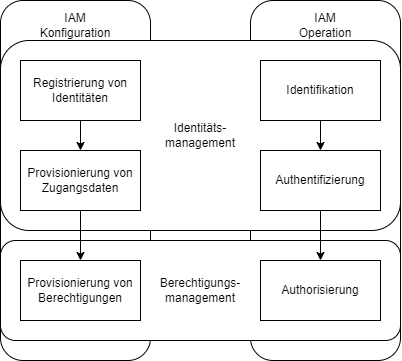
\includegraphics[width=0.6\textwidth]{assets/iam-phases.png}
  \label{fig:iamphases}
  \caption{Phasen des Identitäts- und Berechtigungsmanagements - In Anlehnung an: A Multi-Layer Security System for Data Access Control, Authentication, and Authorization von Tamanna Kaiser und Rafa Siddiqua}
\end{figure}
\subsection{Erkenntnisse im Kontext von IT-GRC}
\begin{itemize}
  \item Die Nutzung von Identitäts- und Berechtigungsmanagement spielt eine zentrale Rolle im unternehmensweiten Risikomanagement. Durch die Steuerung welche logischen Identitäten auf welche Ressourcen zugreifen kann können eine Vielzahl an beabsichtigter und unbeabsichtigter Sicherheitsrisiken minimiert werden.
\end{itemize}
\section{Methoden, Technologien und Tools}
\label{sec:existing}
\subsection{Betriebliche Motivation}
\subsection{Standards}
\paragraph{BSI}
Das Bundesamt für Sicherheit der Informationstechnik (BSI) definiert den IT-Grundschutz. Dieser besteht aus den BSI-Standards und dem IT-Grundschutz-Kompendium. In BSI-Standard 200-1 werden Sicherheitsmaßnahmen definiert die zur Behandlung der Risiken geeignet sind, in diesen Sicherheitsmaßnahmen wird das Identitäts- und Berechtigungsmanagement als Sicherheitsmaßnahme aufgeführt. In Bezug auf den BSI-Standard definiert das IT-Grundschutz-Kompendium Prozessbausteine zur Umsetzung des ISMS. Hier wird im Prozessbaustein \glqq{}ORP.4 Identitäts- und Berechtigungsmanagent\grqq{} auf verschiedene Anforderungen für die Umsetzung von Identitäts- und Berechtigungsmanagement eingegangen. Kapitel 3.1 definiert Basis-Anforderungen welche umgesetzt werden müssen. Kapitel 3.2 definiert Standard-Anforderungen welche umgesetzt werden sollten. Kapitel 3.3 definiert Anforderungen welche bei erhöhtem Schutzbedarf umgesetzt werden sollten. Zusätzlich zu ORP.4 gibt es das Dokument \glqq{}Umsetzungshinweise zum Baustein: ORP.4. Identitäts- und Berechtigungsmanagement\grqq{} welches spezifische Maßnahmen definiert.~\cite{orp4}
\paragraph{ISO 27001 Annex A.9}
ISO 27001 definiert mit Anhang A.9 Kontrollen für das Identitäts- und Berechtigungsmanagement. Das Kapitel ist in die Unterkapitel \glqq{}9.1 Geschäftsanforderungen an die Zugangssteuerung\grqq{}, \glqq{}9.2 Benutzerzugangsverwaltung\grqq{}, \glqq{}9.3 Benutzerverantwortlichkeiten\grqq{} und \glqq{}9.4 Zugangssteuerung für Systeme und Anwendungen\grqq{} unterteilt. Die Maßnahmen des oben erwähnten IT-Grundschutz-Kompendiums eignen sich zur Umsetzung der ISO 27001 Kontrollen. Eine Gegenüberstellung des Anhangs A.9 zu den Prozessbausteinen lässt sich im Dokument \glqq{}Zuordnungstabelle: Zuordnung ISO/IEC 27001 zum IT-Grundschutz\grqq{} finden. Mithilfe dieses Dokuments kann eine ISO 27001 Zertifizierung auf Basis von IT-Grundschutz umgesetzt werden.~\cite{bsi2023basis}
\paragraph{ISO/IEC 24760}
Eine speziell für Identitätsmanagement erstellte Norm ist ISO/IEC 24760. Hierbei werden Konzepte und operative Strukturen zur korrekten Umsetzung von Identitätsmanagement definiert.~\cite{isoiec24760}
\paragraph{NIST 800-53A}
Das National Institute of Standards and Technology (NIST) publizierte die \glqq{}NIST Special Publication 800-53A - Assessing Security and Privacy Controls in Information Systems and Organizations\grqq{}. Dieses Dokument stellt Prozesse und Methoden für die Bewertung von Sicherheits- und Datenschutzmaßnahmen vor. Im Kapitel \glqq{}Security and Privacy Assessment Procedures\grqq{} wird im Unterkapitel 4.1 \glqq{}Access Control Family (AC)\grqq{} auf Zugangskontrolle und im Unterkapitel 4.7 \glqq{}Identification and Authentication Family (IA)\grqq{} auf Identifizierung und Authentifizierung eingegangen.
\subsection{Methoden und Prozesse}
\subsubsection{Identitäts Lebenszyklus}
Ein zentraler Prozess welcher im Rahmen des Identitätsmanagements definiert und umgesetzt werden muss ist der Identitäts Lebenszyklus. Dieser enthält die grundlegenden Elemente Geburt, Leben, Änderung, Tod und Governance. Der Prozess ist in \cref{fig:idlc} dargestellt und wird nachfolgend genauer beschrieben.~\cite{bertino2010identity}
\begin{figure}[H]
  \centering
  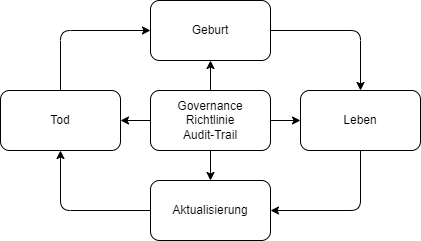
\includegraphics[width=0.6\textwidth]{assets/idlc.png}
  \label{fig:idlc}
  \caption{Identity Life Cycle - In Anlehnung an: Identity Management Concepts, Technologies, and Systems von Elisa Bertino und Kenji Takahashi}
\end{figure}
\paragraph{Geburt}
\subparagraph{Festlegung und Überprüfung von Attributen}
Der erste Schritt in der Geburt einer Identität ist die Sammlung relevanter Attribute wie Name, Geburtsdatum, Wohnsitz, Rolle im Unternehmen etc. und Überprüfung dieser.~\cite{bertino2010identity}
\subparagraph{Festlegen von Anmeldeinformationen}
Um dem Subjekt Zugriff auf die provisionierte Identität zu geben müssen Bezeichner (z.B. E-Mail Addressen oder Nutzernamen) und geeignete Verfahren zur Authentifikation festgelegt werden. So werden in diesem Schritt z.B. Einmalpasswörter für die initiale Anmeldung vergeben oder der Fingerabdruck der zu authentifizierenden Person gespeichert.~\cite{bertino2010identity}
\subparagraph{Abschließende Erstellung}
Nachdem alle relevanten Informationen zur Erstellung der Identität gesammelt wurden kann die Identität erstellt werden.~\cite{bertino2010identity}
\paragraph{Leben}
\subparagraph{Authentifizierung}
Die Authentifizierung der eignenen Identität ermöglicht die gesicherte Nutzung von Ressourcen.~\cite{bertino2010identity}
\subparagraph{Weitergabe von Informationen}
Verfahren zur Weitergabe von Informationen sind ein zentraler Aspekt beim Ausleben einer digitalen Identität.~\cite{bertino2010identity}
\paragraph{Aktualisierung}
\subparagraph{Änderungen}
Bei Änderung von Attributen wie z.B. Rollen im Unternehmen, Wohnort oder Namensänderung müssen die Attribute schnellstmöglich aktualisiert werden um die Integrität dieser zu gewährleisten. Zugangsdaten wie neu ausgestellte Zertifikate oder geänderte Passwörter müssen ebenso aktualisiert werden um die Authentifizierung zu gewährleisten.~\cite{bertino2010identity}
\paragraph{Tod}
\subparagraph{Entzug von Zugangsrechten}
Bei der Kündigung oder Beurlaubung von Mitarbeitern oder bei der Dekommisionierung von Systemen muss der Zugriff auf Ressourcen aufgehoben werden um Sicherheitsrisiken zu verhindern. In diesem Szenario ist es jedoch auch wichtig die Identitätsinformationen weiterhin zu persistieren um für zukünftige Untersuchungen wie z.B. des Audit-Trails eine Zuordnung zu haben.~\cite{bertino2010identity}
\paragraph{Governance}
\subparagraph{Richtlinien}
Die Administration, Nutzung und Weitergabe von Identitätsinformationen muss klar durch Richtlinien definiert sein.~\cite{bertino2010identity}
\subparagraph{Audit Trail}
Jegliche Transaktionen bezüglich Zugriff, Änderung oder Weitergabe von Identitätsinformationen sollten aufgezeichnet werden um die Rückverfolgbarkeit zu gewährleisten.~\cite{bertino2010identity}
\subsection{Technologien und Tools}
IAM Tools ersetzen nicht die Einhaltung von Standards und die sorgfältige Planung von IAM Prozessen. Sie sind jedoch hilfreiche Werkzeuge zur technischen Umsetzung von IAM. So gibt es einige standarisierte Technologien die bei der Implementierung von Identitäts- und Berechtigungsmanagement angewendet werden können. Zur konkreten Umsetzung in Organisationen gibt einige quelloffene Lösungen und von den großen Technologiekonzernen wie Microsoft, SAP, IBM, Oracle werden kommerzielle Lösungen angeboten. Im Folgenden werden einige standartisierte Technologien und Produkte vorgestellt welche bei der Umsetzung von CIAM und IAM verwendet werden.
\subsubsection{Standardisierte Technologien}
\paragraph{SAML}
SAML ist ein weit verbreiteter Standard zur Umsetzung von Sicherheits-Assertationen. Mit SAML wird ein XML Format definiert welches zur Authentifizierung und Authorisierung von Nutzern verwendet werden kann. Im Kontext von SAML werden verschiedene Begrifflichkeiten definiert.~\cite{hughes2005security}
\begin{itemize}
  \item Assertation - Eine Assertation über die Charakteristiken und Attribute eines Subjekts. So z.B. die Zugehörigkeit zu einer Gruppe oder der Besitz eines Attributs.
  \item Identity Provider (IdP) - Der Server der für die eigentliche Bearbeitung der Assertation zuständig ist. Er erhält die Anfrage und leitet die Antwort an den Service Provider weiter.
  \item Service Provider (SP) - Das Ziel der Authentifizierung/Authorisierung, dieser stellt eine Ressource/Service zur Verfügung.
\end{itemize}
\paragraph{OAuth}
OAuth ist eine verbreiteter Standard zur delegierten Zugriffskontrolle welcher in RFC 6749 definiert wird. OAuth ist ein Framework welches das Problem der Autorisierung Dritter lößt. Somit müssen keine sensiblen Informationen wie Passwörter mit Dritten geteilt werden um ihnen Zugriff auf eine Ressource zu geben. Im Kontext des Standards werden folgende Begriffe definiert.
\begin{itemize}
  \item Ressourcenbesitzer - Eine Entität welche die Ressource besitzt und Zugriff gewähren kann
  \item Ressourcenserver - Ein Server welcher die Ressource hostet und auf Anfragen mittel Zugriffstokens reagieren kann
  \item Klient - Eine Anwendung welcher für Ressourcen authorisiert ist und Anfragen an den Ressourcenserver senden kann
  \item Authorisierungsserver - Ein Server welcher Zugriffstokens im Name des Ressourcenbesitzers an den Klient ausstellen kann
\end{itemize}
Der Ablauf des Protokolls ist in Grafik~\cref{fig:oauth} abgebildet.~\cite{rfc6749}
\begin{figure}[H]
  \centering
  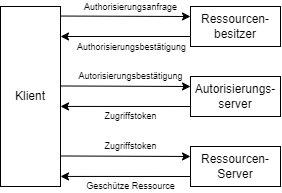
\includegraphics[width=0.6\textwidth]{assets/oauth.png}
  \label{fig:oauth}
  \caption{Protokoll OAuth 2.0 - [Basierend auf RFC 6749]}
\end{figure}
\paragraph{OpenID}
OpenID Connect (OIDC) ist ein Standard für Föderierte Authentifizierung welches die veraltete OpenID 2.0 Spezifikation ablößt.
\subsubsection{IAM Lösungen}
\paragraph{Shibboleth}
Shibboleth ist eine quelloffene Lösung zur Umsetzung von SSO. Shibboleth basiert auf SAML und setzt daher das Prinzip der Föderierten Identität mittels IdP und SP um. Die Technologie setzt sich aus 3 Software Paketen zusammen. IdP, SP und Embedded Discovery Service. Der Embedded Discovery Service erlaubt einem SP mehrere IdP's zur Verfügung zu stellen.
\paragraph{IBM Security Verify}
IBM bietet mit dem Produkt \glqq{}IBM Security Verify\grqq{} eine Cloud basierte Lösung zum Identitäts- und Berechtigungsmanagement an. Dieses Produkt bietet umfangreiche Funktionalitäten wie SSO, MFA, KI gestütze Risikobewertung von Zugriffen und Identitätsanalyse, d.h. die Analyse von Identitäten und Berechtigungen zum Zweck der Identifizierung von Abweichungen.
\paragraph{Microsoft Entra ID}
Microsoft bietet mit dem Produkt \glqq{}Microsoft Entra ID\grqq{} eine Cloud basierte Lösung zum Identitäts- und Berechtigungsmanagement von Microsoft und drittpartei Diensten an. Dieses Produkt bietet Funktionen wie z.B. Multi-Faktor-Authentifizierung mittels Microsoft Authenticator.
\paragraph{SAP Cloud Identity Access Governance}
SAP bietet mit dem Produkt \glqq{}SAP Cloud Identity Access Governenace\grqq{} eine Cloud basierte Lösung zum Identitäts- und Berechtigungsmanagement an. SAP selbst schreibt dem Produkt eine intuitive Bedienung, hohe Anpassbarkeit und skalierbare Funktionen zu.
\paragraph{Okta Inc.}
Das Unternehmen Okta Inc. ist ein in den USA ansässiges Unternehmen welches sich auf IAM spezialisiert hat. Mit rund 6000 Mitarbeitern und mehr als einer Milliarde US-Dollar an Umsatz ist es ein führender Hersteller von IAM Produkten. Vom Unternehmen werden 2 Produkte angeboten. Customer Identity Cloud und Workforce Identity Cloud. Customer Identity Cloud ist eine Lösung zum Customer Identity Management, d.h. es ermöglicht die sichere Verwaltung und Authentifizierung von Kunden-Identitäten. Workforce Identity Cloud ist eine Lösung zum Unternehmensinternen Identitätsmanagement.
\subsection{Erkenntnisse im Kontext von IT-GRC}
\begin{itemize}
  \item Im Rahmen von Normen wie der ISO 27001 spielt die Umsetzung von IAM eine zentrale Rolle.
  \item Professionelle IAM Lösungen können durch eine Vielzahl an Funktionalitäten dazu beitragen Identitäts- und Berechtigungsmanagement effizient umzusetzen.
\end{itemize}
\section{Betriebliches Identitäts- und Berechtigungsmanagement}
\label{sec:betrieb}
\subsection{Überblick}
\subsection{Organisatorische Aspekte}
Im Rahmen der Ausarbeitung eines IAM Konzepts im Unternehmen müssen hierbei klare Verantwortlichkeiten, Prozesse und Technologien definiert werden. Die relevanten Organisationseinheiten zum Identitäts- und Berechtigungsmanagement werden im Folgenden vorgestellt.
\paragraph{Führungebene}
IAM fällt unter die Domäne der Informationssicherheit, benötigt jedoch gegebenfalls umfangreiche IT Infrastruktur und Produkte. Auf der Führungsebene im Unternehmen sind daher der Chief Information Security Officer (CISO) und der Chief Information Officer (CIO) für die Umsetzung des Identitäts- und Berechtigungsmanagement verantwortlich.~\cite{azhar2014economics}\cite{baldwin2009using} Im Fall von umfangreichen Anforderungen an das System kann die Umsetzung des IAM ein ganzes Team benötigen.~\cite{mohammed2011identity}
\paragraph{Helpdesk}
Der Helpdesk ist im Unternehmen eine zentrale Anlaufstelle für Probleme mit der Authentifizierung wie vergessener Passwörter oder fehlender Berechtigungen. So wurde bei Umfragen festgestellt dass je nach Unternehmen 10-66 \% aller Helpdesk Tickets aufgrund von vergessener Passwörter erstellt werden.~\cite{ylen2004centralized}\cite{tsolkas2017} Ein wichtiger Aspekt hierbei ist die Einhaltung fester Prozesse welche mögliche Angriffe durch Social Engineering verhindern.~\cite{wood2005implementing}
\paragraph{Personalmanagement}
Eine Zentrale Rolle in der Provisionierung und Änderung von Identitäten spielt das Personalmanagement. Dieses ist für die erstmalige Erstellung der Identitäten, der Ausgabe von Authentifizierungsinformationen, der Vergabe von Rollen für rollenbasierte Zugriffskontrolle und der Deprovisionierung bei Beurlaubung und Kündigung zuständig.~\cite{YOUNG20045}\cite{mohammed2017systematic}
\subsection{Technische Aspekte}
Für die Umsetzung von Identitäts- und Berechtigungsmanagement im Betrieb bieten sich die Lösungen der namhaften Hersteller wie Microsoft, SAP oder Okta an. Dies sind ausgereifte Lösungen mit einer Vielzahl an Funktionalitäten die die Umsetzung des Identitäts- und Berechtigungsmanagements unterstützen. Während der traditionelle Ansatz die Nutzung von On-Premise Services war bewegt sich die IAM Industrie in Richtung von SaaS Modellen. Im Kontext von IAM werden diese Lösungen als IDaaS bezeichnet.~\cite{kunz2014analyzing}
\subsection{Wirtschaftliche Aspekte}
Die Signifikanz von Identitäts- und Berechtigungsmanagement in Unternehmen tiefgreifend. Es lassen sich 4 Aspekte identifizieren. Security, Produktivität, Compliance und Kundenerlebnis.~\cite{mont2010economics}\cite{azhar2014economics} Diese 4 Aspekte sind im Folgenden aufgeführt.
\paragraph{Security}
Der wirtschaftliche Schaden der durch Datendiebstahl und unautorisierter Kontrolle entstehen kann ist immens.~\cite{azhar2014economics} Wenn ein Mitarbeiter eine Vielzahl an Passwörtern für die unternehmensinternen/unternehmensexternen Dienste verwalten muss kann dies zur unsachgemäßen Handhabung führen - so z.B. Notizen mit Passwörtern oder die Verwendung von schwachen Passwörtern, dies erhöht die Wahrscheinlichkeit von Sicherheitrisiken.~\cite{haag2012selecting}~\cite{azhar2014economics} Im Jahr 2017 fiel Deloitte einem Cyberangriff zum Opfer. Hierbei wurden Nutzernamen, Passwörter, IP Addressen und sensible Unternehmensinformationen von 244.000 Mitarbeitern und Kunden geklaut. Grund für den Cyberangriff war ein Administratoraccount ohne Zugriffsbeschränkungen welcher nur mittels Passwort, ohne MFA geschützt war.~\cite{deloitte2017} Mittels fest definierter Prozesse des Identity Management Life Cycles und Audit dieses können Risiken für ähnliche Angriffe minimiert werden.
\paragraph{Produktivität}
Im vorherigen Abschnitt wurde die wirtschaftliche Signifikanz von Identitäts- und Berechtigungsmanagement aufgezeigt. Dies kann jedoch einen negativen Einfluss auf die Produktivität von Mitarbeitern haben. So führt z.B. die Verwendung von mehreren verschiedenen Systemen, alle mit unterschiedlichen Authentifizierungsverfahren dazu dass Mitarbeiter verschiedene Passwörter verwalten müssen oder sich in jedem System separat authentifizieren müssen. Mit der Anwendung von SSO Verfahren lässt sich dieser Aufwand auf ein Minimum reduzieren.~\cite{radha2012survey}~\cite{haag2012selecting} Während die Umsetzung des Principle of Least Privilege wünscheswert ist können schlecht konfigurierte Zugriffsberechtigungen dazu führen dass Mitarbeiter ihre Arbeit unterbrechen müssen um neue Rechte anzufordern. Dies kann unter Umständen zu teuren Verzögerungen im direkten Arbeitsablauf adminstrativer oder operativer Aufgaben führen.~\cite{weishaupl2015towards}
\paragraph{Kundenerlebnis}
Im Kontext des Customer IAM führen ungeeignete IAM Lösungen zu erhöhter Komplexität für den Nutzer. Eine strikte Umsetzung von starken Passwörtern oder die Nutzung einer weiteren MFA-App kann für den Kunden abschreckend sein. Somit steigt der Kunde möglicherweise zur Konkurrenz um.~\cite{azhar2014economics} Durch das Anbieten von SSO mittels externer Dienste lässt sich die Komplexität und das Risiko von Sicherheitsproblemen reduzieren.
\paragraph{Compliance}
\subparagraph{EuroSOX}
Die Richtlinie 2006/43/EG, durch den direkten Bezug zum Sarbanes Oxley Act auch EuroSOX genannt fordert im Rahmen des Internen Kontrollsystems nach einer Berechtigungsvergabe und Funktionstrennung im Unternehmen. Dies stellt eine direkte Forderung für Identitäts- und Berechtigungsmanagement dar.~\cite{conta2017leitfaden}
\subparagraph{KonTraG}
Das KonTraG fordert Unternehmen auf ein Risikomanagementsystem zu implementieren. Unauthorisierter Zugriff auf sensible Daten und Geschäftsprozesse kann in diesem Kontext als Risiko aufgefasst werden. D.h. es besteht eine indirekte Forderung nach Identitäts- und Berechtigungsmanagement.~\cite{conta2017leitfaden}
\subparagraph{BDSG}
Im BDSG nimmt Identitäts- und Berechtigungsmanagement eine zentrale Rolle ein.
\begin{itemize}
  \item Zutrittskontrolle, Zugriffskontrolle: Systeme die personenbezogene Daten verarbeiten müssen vor unauthorisiertem Zutritt und Zugriff geschützt werden.~\cite{conta2017leitfaden} Dies stellt eine direkte Forderung für physische und logische Berechtigungskontrollen dar.
  \item Weitergabekontrolle: Beim Transport von personenbezogenen Daten die Vertraulichkeit und Integrität der Daten gewährleistet wird und dass jegliche Transaktionen protokolliert werden müssen.~\cite{conta2017leitfaden} Dies stellt eine direkte Forderung für Audit-Trails und Berechtigungskontrollen dar.
  \item Eingabekontrolle: Bei der Erfassung von personenbezogenen Daten muss die Nachvollziehbarkeit des Ursprungs gewährleistet sein.~\cite{conta2017leitfaden} Dies stellt eine direkte Forderung für Audit-Trails dar.
\end{itemize}
\paragraph{EU-DSGVO}
Die DSGVO stellt verschiedenste Forderungen für die sichere Erhebung, Speicherung und Verarbeitung von personenbezogener Daten.~\cite{Hindle_2020}
\begin{itemize}
  \item Artikel 5 - Grundsätze für die Verarbeitung personenbezogener Daten - Paragraph 1.f: Die Integrität und Vertraulichkeit personenbezogene Daten muss gewährleistet sein.~\cite{eu2016} Somit müssen geeignete Verfahren zur Zutritts und Zugriffskontrolle vorhanden sein.
  \item Artikel 15 - Auskunftsrecht der betroffenen Person - Paragraph 3: Das betroffene Person über die Daten erhoben wurde hat das Recht Auskunft über alle personenbezogenen Daten anzufordern.~\cite{eu2016} Hierbei sind geeignete Prozesse im Rahmen des Identitätsmanagements zu definieren. Diese müssen durch geeignete Authentifizierungsverfahren geschützt werden um die Vertraulichkeit der Weitergabe zu gewährleisten.
  \item Artikel 17 - Recht auf Löschung - Paragraph 1: Die betroffene Person hat das Recht eine Forderung für die unverzügliche Löschung der Daten einzureichen.~\cite{eu2016} Hierbei sind geeignete Prozesse im Rahmen des Identitätsmanagements zu definieren.
\end{itemize}
\subsection{Erkenntnisse im Kontext von IT-GRC}
\begin{itemize}
  \item Die Umsetzung von IAM kann kostspielig sein denn das Management und die eingesetzten Technologien sind teuer. Rechtlichen Vorgaben sind jedoch nicht optional und die Risiken von fehlendem IAM können enorm sein.
\end{itemize}
\section{Fazit}
\subsection{Zusammenfassung}
\subsection{Beantwortung der Forschungsfragen}
\paragraph{Identität und Identitätsmanagement}
Eine (digitale) Identität ist eine Menge von Attributen und Rollen, inklusive Bezeichner und Zugangsdaten zur Authorisierung. So kann eine Identität eine Person, ein IT-System oder eine Anwendung darstellen. Eine Identität kann einer Entität, also einer Person oder einer Organisation zugeordnet werden. Das Identitätsmanagement ist zuständig für die Festlegung von Prozessen zur Verwaltung, Authentifizierung und Überwachung von Identitäten.
\paragraph{Berechtigung und Berechtigungsmanagement}
Eine Berechtigung ist eine Kombination aus zu berechtigender Ressource und zu berechtigender Operation auf diese Ressource. Berechtigungsmanagement bezeichnet die Prozesse für die Zuweisung, Kontrolle, Überwachung und Entzug von Berechtigungen sowie der Überwachung dieser Prozesse.
\paragraph{Welche Standards, Methoden, Technologien und Tools lassen sich differenzieren?}
Die ISO 27001 Norm in Kombination mit dem IT-Grundschutz des BSI's stellt einen Goldstandard in der Informationssicherheit in Organisationen dar. Ein wichtiger Aspekt einer ISO 27001 Zertifizierung ist die Zugriffskontrolle.  Es haben sich einige standardisierte Verfahren zur Umsetzung von Identitäts- und Berechtigungsmanagement etabliert, so z.B. SAML, OAuth, OpenID Connect. Es gibt eine Vielzahl an Anbietern welche IAM Lösungen anbieten. Beispiele für große Hersteller sind Microsoft, IBM, SAP und Okta.
\paragraph{Welche Aufgaben und Prozesse sind im Kontext von Identitäts- und Berechtigungsmanagement zu bearbeiten?}
Die grundlegenden Aufgaben und Prozesse des Identitäts- und Berechtigungsmanagements sind:
\begin{itemize}
  \item Provisionierung, Änderung und Deprovisionierung von digitalen Identitäten und Berechtigungen
  \item Technische Umsetzung der Infrastruktur zur Speicherung der relevanten Informationen, der Authentifizierung und der Authorisierung
  \item Identifikation von rechtlichen Aspekten und Standards, Planung von Prozessen zur Einhaltung dieser
  \item Auditierung aller Prozesse zur Identifikation von Abweichungen und Speicherung von Informationen im Rahmen der Rückverfolgbarkeit von Transaktionen
\end{itemize}
\paragraph{Welche betrieblichen Anwendungsfälle zeigen die Bedeutung des Identitäts und Berechtigungsmanagements auf?}
\paragraph{Wie wird das Identitäts und Berechtigungsmanagement im Kontext der Sicherheit in der Informationstechnik eingesetzt?}
Das Identitäts- und Berechtigungsmanagement wird eingesetzt um Zugriffe auf schützenswerte Ressourcen einzuschränken. Dies geschieht durch geeignete Authentifizierungs und Authorisierungsverfahren.
\paragraph{Zuständigkeit für Identitäts- und Berechtigungsmanagement}
Für die Planung und Umsetzung der Prozessen des Identitäts- und Berechtigungsmanagements ist im Unternehmen der CIO verantwortlich. Dieser wird ggf. durch den CISO unterstützt denn Identitäts- und Berechtigungsmanagement ist ein sicherheitskritischer Prozess. Operativ involviert sind die Personalverwaltung und der Helpdesk. Die Personalverwaltung ist zuständig für die Erstellung, Änderung und Löschung von Identitäten und Rollen. Der Helpdesk ist die Anlaufstelle für Probleme bei der Nutzung von Identitäts- und Berechtigungsmanagement-Systemen und bei Incidents.
\newpage
\section{Eidesstattliche Versicherung}
\newpage
\printbibliography[notkeyword={quelle}, title={Literaturverzeichnis}]
\newpage
\printbibliography[keyword={quelle}, title={Quellenverzeichnis}]
\newpage
\listoffigures
\end{document}